\documentclass[12pt,a4paper,oneside]{article}

\usepackage[utf8]{inputenc}
\usepackage[italian]{babel}
\usepackage{graphicx}
\usepackage{float}
\usepackage{booktabs}
\usepackage{hyperref}
\usepackage{geometry}
\usepackage{longtable}
\usepackage{tabularx}
\geometry{a4paper, top=3cm, bottom=3cm, left=3cm, right=3cm}

% --- Configurazione Links ---
\hypersetup{
    colorlinks=true,
    linkcolor=black,
    filecolor=magenta,      
    urlcolor=blue,
}

\begin{document}

\begin{titlepage}
    \begin{center}
        \large
        ALMA MATER STUDIORUM - UNIVERSITÀ DI BOLOGNA \\
        \vspace{0.5cm}
        CAMPUS DI CESENA\\
        \vspace{0.5cm}
        CORSO DI LAUREA TRIENNALE IN INGEGNERIA E \\
        SCIENZE INFORMATICHE
        \vspace{3.5cm}
        
        \Large
        \textbf{Relazione di Tirocinio Curricolare} \\
        \vspace{1cm}
        \huge
        \textbf{Sviluppo di un'infrastruttura simulata in ambito sanitario} \\

        \vspace{1cm}
        \large
        A.A. 2025-2026

        \vspace{3.5cm}
        
        \noindent
        \begin{minipage}[t]{0.45\textwidth}
            \large
            \textbf{Tirocinante:}\\
            Justin Carideo
        \end{minipage}
        \hfill
        \begin{minipage}[t]{0.5\textwidth}
            \large
            \raggedleft
            \textbf{Tutor Didattico:}\\
            Prof. Alessandro Ricci\\
            \vspace{0.4cm}
            \textbf{Co-supervisore:}\\
            Ing. Angelo Croatti
        \end{minipage}
        
        \vfill
        \hrule height 0.4pt
        \vspace{0.2cm}
        \large
        \textbf{Periodo di svolgimento:} 02/03/2026 -- 09/06/2026
    \end{center}
\end{titlepage}

\tableofcontents
\newpage

% --- SEZIONE 1 ---
\section{Introduzione}
Nel contesto sanitario, l'efficacia della fase di soccorso extra-ospedaliera è
strettamente legata all'adozione di metodologie rigorose e alla rapidità di
intervento. Attualmente si utilizzano sistemi software in grado di supportare
questo modus operandi, ma sorge l'esigenza di far evolvere tali strumenti
sfruttando le tecnologie più moderne per ottimizzare l'intero processo di
gestione delle emergenze.

Al momento, l'AUSL Romagna adotta un sistema mobile denominato 
\textbf{Trauma Tracker}, progettato per tracciare ogni manovra ed evento clinico-logistico 
che si verifica durante il soccorso di pazienti con trauma grave nella fase
pre-ospedaliera. I soccorritori sul campo hanno a disposizione un dispositivo
mobile equipaggiato con un'applicazione dedicata alla registrazione tempestiva
delle procedure effettuate. Tale applicazione interagisce sia con un backend
centralizzato, deputato al mantenimento dello storico dei dati, sia con
trasmettitori radio basati su tecnologia \textit{Beacon BLE}, in grado di
comunicare direttamente con i dispositivi medici di tracciamento dei parametri
vitali.

Questa analisi del sistema preesistente permette di delineare le linee
guida fondamentali che il presente progetto deve ereditare ed estendere. In primo
luogo, la tracciabilità degli eventi deve evolvere, attraverso l'integrazione
di un ecosistema IoT, verso un monitoraggio puramente real-time; in secondo
luogo, i dati raccolti devono consentire la creazione di un sistema di analisi
a posteriori, abilitando una retrospettiva accurata delle dinamiche di soccorso.
Di conseguenza, si rende necessario individuare un paradigma tecnologico capace
di fondere queste due anime fondanti del progetto Trauma Tracker e la scelta più
appropriata è stata individuata nei \textit{Digital Twin}.

L'analisi dei requisiti e la modellazione del sistema partono dall'adozione
della metodologia del \texttt{Domain-Driven Design} (DDD), un approccio strategico
fondamentalmente per far sì che qualunque esperto del dominio clinico sia
in grado di interpretare e comprendere ogni componente dell'architettura
software creata, definendo un \textit{Ubiquitous Language} condiviso.
L'obiettivo del tirocinio si focalizza, pertanto,
sulla progettazione di tale infrastruttura abilitante, ponendo le basi
architetturali che verranno successivamente estese ed
approfondite nel progetto di tesi.

La problematica principale nello sviluppo di un simile ecosistema risiede
nell'impossibilità di validare il software in un contesto reale di emergenza, 
scenario che risulterebbe estremamente rischioso e controproducente. In tal senso, 
si è optato per la \textbf{simulazione} come tecnologia chiave per aggirare questi 
limiti operativi. L'integrazione di un motore di simulazione consente non solo di 
testare la reattività e la robustezza dell'architettura IoT in totale sicurezza, 
ma costituisce anche uno strumento vivo per l'apprendimento e la comprensione 
approfondita delle dinamiche complesse del dominio sanitario.

\section{Tecnologie}
Il raggiungimento degli obiettivi prefissati ha richiesto l'integrazione di 
diverse piattaforme software e protocolli di rete, volti a garantire il 
corretto disaccoppiamento dei componenti e la modularità dell'infrastruttura.

\subsection{AnyLogic}
AnyLogic è un motore di simulazione multifunzionale scritto in Java che supporta i principali 
paradigmi di modellazione: \textit{Agent-Based}, \textit{Discrete Event} e 
\textit{System Dynamics}. All'interno del progetto, l'approccio orientato 
agli agenti è stato sfruttato per definire la granularità comportamentale 
e spaziale delle entità fisiche coinvolte (pazienti, equipaggi, veicoli di 
soccorso) all'interno di un ambiente continuo basato su mappe GIS (Geographic 
Information System) reali della regione Romagna.

\subsection{Protocollo MQTT}
Il protocollo MQTT (Message Queuing Telemetry Transport) è uno standard di 
messaggistica Pub/Sub (Publish/Subscribe) leggero, progettato per contesti 
IoT con risorse di rete limitate. La sua architettura basata su broker 
centralizzati garantisce il totale disaccoppiamento spaziale e temporale 
tra il Layer di Simulazione e gli applicativi esterni, consentendo di manipolare
 lo stato del modello attraverso l'\textit{injection} di dati strutturati e 
 asincroni in formato JSON.

\subsection{Eclipse Paho}
Eclipse Paho è una libreria open-source che fornisce implementazioni client 
affidabili per i protocolli MQTT. Nel contesto del progetto, le API Java di 
Paho sono state integrate direttamente all'interno delle classi custom e degli 
agenti di AnyLogic. Ciò ha permesso al modello simulativo di agire nativamente 
come un client MQTT in grado di sottoscriversi ai topic di comando e di pubblicare 
in tempo reale la telemetria geografica e i cambi di stato operativo.

\subsection{Eclipse Mosquitto}
Eclipse Mosquitto è un broker open-source che implementa le specifiche
del protocollo MQTT. All'interno dell'architettura, Mosquitto funge
da pilastro per lo scambio dei messaggi, prendendosi carico del routing
dei payload JSON provenienti dai sistemi di iniezione dati o generati 
dalla simulazione stessa, garantendo latenze minime e alta affidabilità 
nella distribuzione degli eventi.

\subsection{Docker e Docker-Compose}
Docker è una piattaforma di containerizzazione che permette di isolare i 
servizi software all'interno di ambienti leggeri e riproducibili denominati 
\textit{container}. Mediante l'utilizzo di Docker-Compose, è stata definita 
e orchestrata l'intera infrastruttura di rete locale (incluso il broker Mosquitto),
 azzerando le discrepanze di configurazione ambientale e isolando l'architettura 
 per i test di deployment.

\subsection{MQTT Explorer}
MQTT Explorer è un client grafico completo per la visualizzazione e l'interazione 
con i broker MQTT. Caratterizzato da una struttura ad albero gerarchica per la 
rappresentazione dei topic, lo strumento è stato impiegato come utility di 
controllo sia per monitorare i flussi di telemetria emessi da AnyLogic, sia 
per validare i meccanismi di iniezione dati attraverso la pubblicazione manuale 
di payload JSON di test.

\section{Attività}
Questa sezione illustra le fasi centrali di progettazione ingegneristica dell'infrastruttura.

\subsection{Ubiquitous Language}
In conformità con le linee guida del \textit{Domain-Driven Design} (DDD),
lo sviluppo dell'architettura è stato preceduto dalla formalizzazione
del linguaggio ubiquitario (\textit{Ubiquitous Language}).
Questa attività mappa i concetti operativi e clinici della fase pre-ospedaliera
(\textit{PreH}) in termini tecnici condivisi tra sviluppatori ed
esperti di dominio.

\begin{longtable}{|l|p{11cm}|}

\caption{Ubiquitous Language PreH} \label{tab:ubiquitous_language} \\

\hline
\textbf{Termine} & \textbf{Definizione} \\
\hline\hline
\endfirsthead

\multicolumn{2}{c}{\tablename\ \thetable{}} \\
\hline
\textbf{Termine} & \textbf{Definizione} \\
\hline\hline
\endhead

\endfoot

\hline
\endlastfoot

Centrale Operativa & Unità operativa che abilita un Soccorritore e un Veicolo di Soccorso (Ambulanza o Elisoccorso) per dirigersi verso il luogo in cui prestare soccorso. \\
\hline
Soccorritore & Unità in grado di operare nel Scenario di Soccorso. Spesso è un volontario o dipendente che ha un addestramento al primo soccorso. Non può fare diagnosi o somministrare farmaci. Può guidare un mezzo (solitamente ambulanze e automediche) e fare manovre base di primo soccorso. \\
\hline
Infermiere & Unità in grado di fare le manovre di soccorso avanzate, sotto protocollo può somministrare farmaci. Collabora con il medico se presente sul mezzo o scenario. Di norma guida l'equipaggio della \textit{India} (Ambulanza Avanzata). \\
\hline
Medico & Unità che ha la massima responsabilità sul target. Può fare diagnosi e somministrare farmaci. Decide la destinazione del Paziente e come gestire il soccorso nello Scenario di Soccorso. \\
\hline
Equipaggio & Insieme di professionisti (Soccorritori, Infermieri, Medici) che si trovano a bordo di un Veicolo di Soccorso. \\
\hline
Veicolo di Soccorso & Mezzo di trasporto (Ambulanza, Automedica o Elisoccorso) che viene utilizzato per muoversi e raggiungere lo Scenario di Soccorso ed eventualmente trasportare il Paziente. \\
\hline
Paziente & Il target che ha subito un trauma grave nel territorio e che necessita di essere soccorso e stabilizzato. \\
\hline
Scenario di Soccorso & Luogo geografico in cui si è verificato l'evento per cui è stato richiesto soccorso. All'interno operano gli Equipaggi. \\
\hline
Cinematica del Trauma & Studio delle forze che hanno colpito il Paziente a seguito di un incidente. Aiuta a comprendere la gravità delle lesioni interne anche in assenza di sintomi evidenti. \\
\hline
Parametri Vitali PreH & Insieme di dati clinici e fisiologici (frequenza cardiaca, pressione arteriosa, saturazione, GCS...) raccolti nello Scenario di Soccorso. \\
\hline
Evento PreH & Qualsiasi azione logistica o clinica (partenza del mezzo, arrivo sullo scenario, inizio di una procedura medica...) che avviene durante la gestione del soccorso. \\
\hline
Report PreH & Documento che raccoglie la cronistoria di tutti gli Eventi PreH e i Parametri Vitali PreH associati a una Missione. \\
\hline
Missione & Insieme di attività coordinate dalla Centrale Operativa, che partono dall'attivazione dell'Equipaggio fino all'Handover. \\
\hline
Handover & Atto formale e di responsabilità penale/medica con cui l'Equipaggio extra-ospedaliero affida il Paziente al personale del Pronto Soccorso. \\
\hline
Pronto Soccorso & Luogo ospedaliero attrezzato per la gestione delle emergenze, punto di arrivo di tutta la fase PreH. \\
\hline

\end{longtable}

Passiamo un utilizzo pratico di questi termini attraverso il \textit{Domain Storytelling}:

\begin{figure}[H]
    \centering
    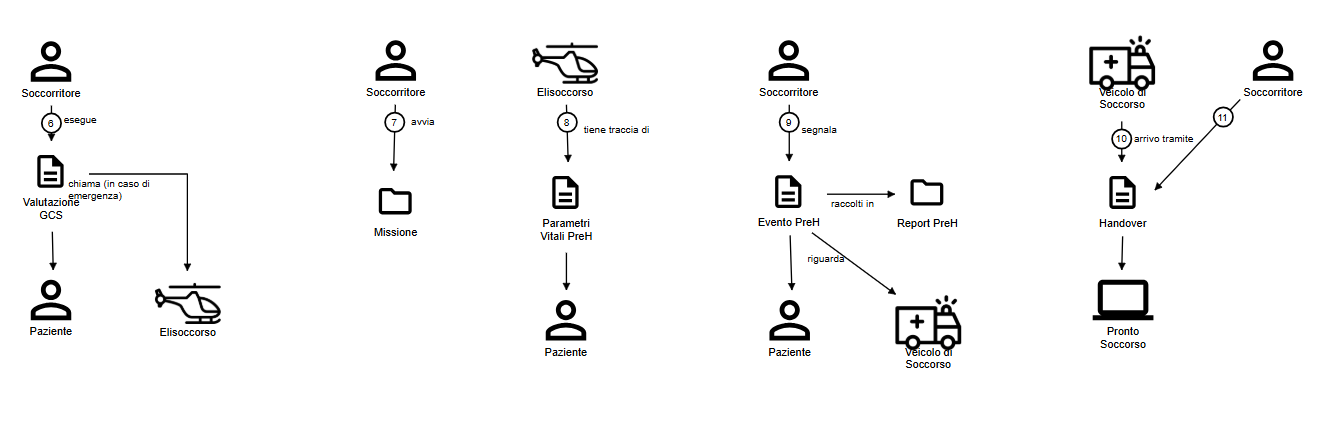
\includegraphics[width=1\textwidth]{img/DS_v1.1.png}
    \caption{Domain Storytelling fase PreH}
    \label{fig:preh1}
\end{figure}

\begin{figure}[H]
    \centering
    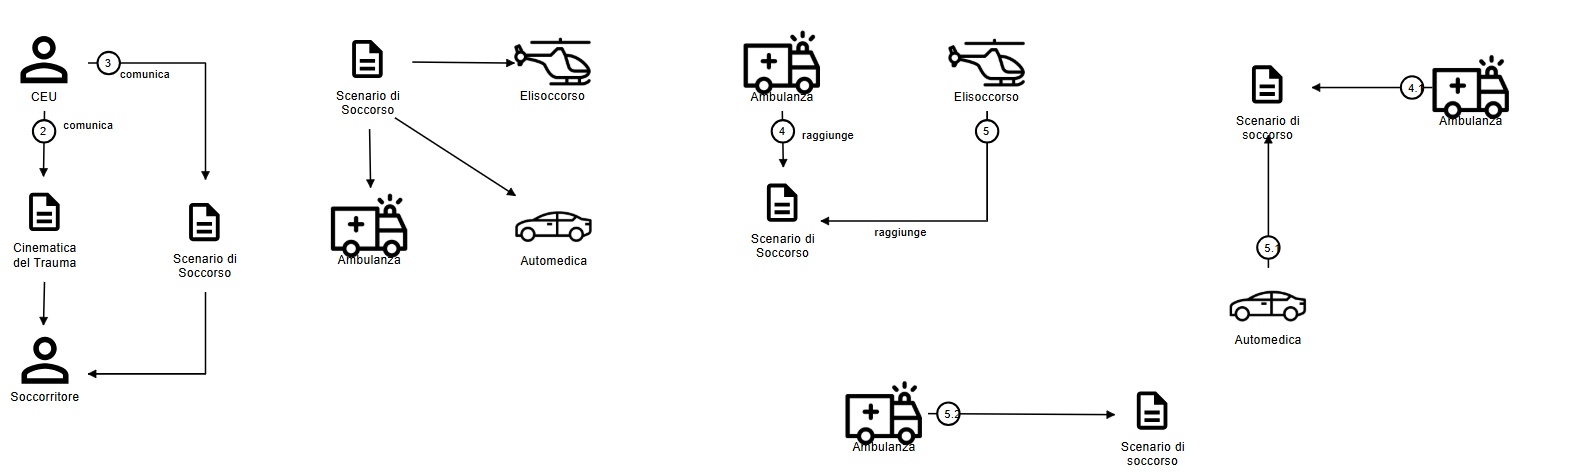
\includegraphics[width=1\textwidth]{img/DS_v1.2.png}
    \caption{Domain Storytelling fase PreH - 2}
    \label{fig:preh2}
\end{figure}

\subsubsection{Descrizione tramite UL}
La \texttt{Missione} si attiva nel momento in cui un cittadino chiama il numero
di emergenza (112/118) per contattare la \texttt{Centrale Operativa}. La Centrale Operativa
segue dei protocolli per effettuare un'analisi preventiva sul \texttt{Paziente}, 
determinando il \texttt{Codice colore}. Dal Codice colore si determina la tempestività
con la quale il Paziente deve essere soccorso.
Una volta determinato il Codice colore, viene scelto un \texttt{Equipaggio} e i mezzi di soccorso.

Il veicolo raggiunge lo Scenario di Soccorso. L'Equipaggio mette in sicurezza 
l'area ed effettua una \texttt{Valutazione Clinica} basata su protocolli standard 
(che include il calcolo del GCS e di altri Parametri vitali).
Questa valutazione conferma la gravità e determina quale sarà l'ospedale 
di destinazione.

La Centrale Operativa monitora attivamente i mezzi in movimento (es. tramite GPS
 e radio) e comunica in quale \texttt{Ospedale} muoversi.
Durante l'intero svolgimento della missione, ogni azione significativa
 (arrivo del mezzo, avvio missione, ecc.) viene registrata come un \texttt{Evento}, dotato di un suo timestamp. 
 Tutti gli Eventi, che riguardano direttamente il Paziente e il veicolo di 
 soccorso coinvolto, vengono raccolti e storicizzati in un \texttt{Report}, un 
 documento (fisico o digitale) che ha valenza sia medica che legale e mostra un 
 resoconto della fase di tracciamento.

La Missione termina con la fase di \texttt{Handover}. Questo è il momento di 
intermezzo che segna il passaggio dalla fase extra-ospedaliera a quella 
intra-ospedaliera, il cui evento scatenante è l'arrivo fisico del veicolo e 
del Paziente al \texttt{Pronto Soccorso}. Il Pronto Soccorso rappresenta il luogo 
di destinazione finale di tutta la fase pre-ospedaliera.


\subsection{Simulazione e Protocollo ODD}
La simulazione è stata documentata attraverso il \textbf{Protocollo ODD} (Overview-Design Concepts-Details), 
utilizzato per descrivere modelli agent-based. Si divide in tre categorie concettuali:
\begin{itemize}
    \item \textbf{Overview}: chi e cosa è presente nel modello.
    \item \textbf{Design Concepts}: principi alla base del comportamento degli agenti.
    \item \textbf{Details}: come è stato implementato il modello.
\end{itemize}

\subsubsection{Overview}
Lo scopo primario del modello è la riproduzione della catena di soccorso
territoriale per valutare l'efficienza di allocazione delle risorse sanitarie, 
calcolare la distribuzione dei tempi di intervento e analizzare l'impatto clinico 
sul \textit{Paziente} vittima di trauma grave. 

I criteri di validazione del modello si basano sull'analisi di due metriche temporali critiche: il 
\textit{Response Time} (dalla ricezione della chiamata all'arrivo del 
mezzo sullo scenario) e il \textit{Total Pre-Hospital Time} (dalla chiamata 
all'avvio dell'fase di \textit{Handover} in Pronto Soccorso).
\vspace{1cm}

Le entità che compongono il modello sono:
\begin{itemize}
    \item \textbf{Ambulance / MedCar / MedHelicopter}: agenti fisici dotati di
    coordinate geografiche dinamiche e degli stati per tracciare lo stato 
    operativo.
    \item \textbf{Patient}: entità dinamica generata a seguito di una segnalazione, 
    caratterizzata da coordinate spaziali statiche di evento, un timestamp di attivazione 
    e un codice di gravità clinica. In questo contesto l'agente simula i sensori che dovrebbero essere attaccati al paziente.
    \item \textbf{Main}: l'agente di contesto che modella il territorio e gli eventi che accadono. 
    Al suo interno risiedono le popolazioni degli agenti e le funzioni 
    di smistamento logistico dei messaggi.
    \item \textbf{CEU}: l'agente che si occupa delle scelte logistiche degli agenti. In particolare
    si occupa di smistare le segnalazioni e di indicare in quale ospedale deve essere portato il paziente.
    \item \textbf{Hospital / StationaryPoint}: sono agenti di contesto che vivono nel \texttt{Main} e servono per orientare gli altri agenti nell'ambiente.
\end{itemize}

Per avere più fedeltà con l'ambiente reale la simulazione ha scala temporale in \textbf{secondi} e una misura spaziale in \textbf{metri}.

Gli agenti con un comportamento hanno i seguenti statechart:
\begin{figure}[H]
    \centering
    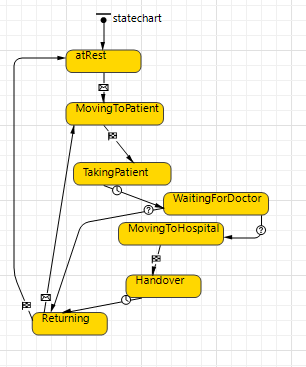
\includegraphics[width=0.4\textwidth]{img/AmbulanceStatechart.png}
    \caption{Statechart di \texttt{Ambulance}}
    \label{fig:ambulanceST}
\end{figure}
\begin{figure}[H]
    \centering
    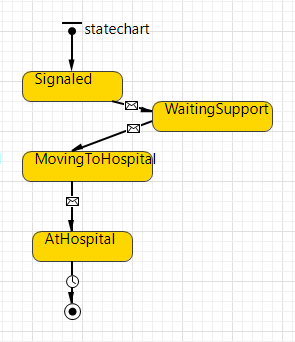
\includegraphics[width=0.4\textwidth]{img/PatientStatechart.png}
    \caption{Statechart di \texttt{Patient}}
    \label{fig:patientST}
\end{figure}
\begin{figure}[H]
    \centering
    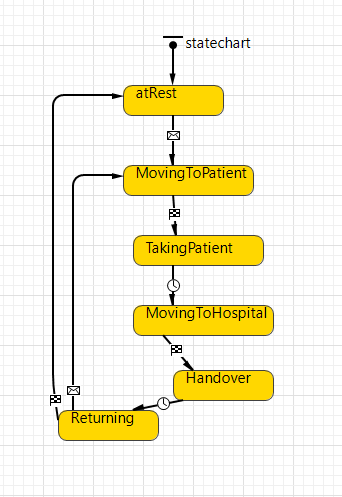
\includegraphics[width=0.4\textwidth]{img/MedHelicopterStatechart.png}
    \caption{Statechart di \texttt{MedHelicopter}}
    \label{fig:medhelicopterST}
\end{figure}
\begin{figure}[H]
    \centering
    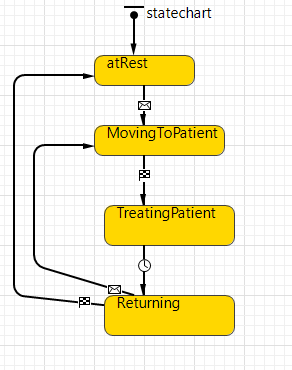
\includegraphics[width=0.4\textwidth]{img/MedCarStatechart.png}
    \caption{Statechart di \texttt{MedCar}}
    \label{fig:medcarST}
\end{figure}


Esiste una parte di \textit{Process Overwiew} che viene delineata in questa fase:
\begin{itemize}
    \item \textbf{Signaling}: generazione di una segnalazione all'interno del \texttt{Main}
    \item \textbf{Dispatching}: \texttt{CEU} indica quali veicoli di soccorso sono coinvolti per il soccorso e dove è avvenuta l'emergenza
    \item \textbf{Caricamento}: i mezzi di soccorso arrivano sul luogo della segnalazione e caricano il paziente all'interno di uno dei veicoli.
    \item \textbf{Trasporto in ospadale}: il paziente viene trasportato in ospedale con gli strumenti più adatti alla gravità della situazione.
    \item \textbf{Handover}: il paziente viene trasportato all'interno dell'ospedale
    \item \textbf{Ritorno}: i mezzi ritornano negli opportuni punti stazionari da cui sono partiti.
\end{itemize}

\subsubsection{Design Concepts}
Le sezioni più importanti in questa fase sono:
\begin{itemize}
    \item \textbf{Basic Principles}: il punto di innesco è la \texttt{CEU}
    che gestisce le segnalazioni e tramite una regola di dispatch seleziona i veicoli da mandare.
    Ogni altro veicolo ha un comportamento autonomo e comunica con gli altri in caso di necessità.
    \item \textbf{Emergence}: i fenomeni emergenti principali sono: 
    \begin{itemize}
        \item I ritardi non dipendono dal numero di mezzi ma dalla lontananza del target e conseguemente dalla locazione dei punti stazionari.
        \item Nonostante i soccorsi extraurbani il tempo di risposta medio tende a convergere.
        \item Congestione ospedale in caso di chiamate simultanee.
    \end{itemize}
    \item \textbf{Adaption}: la \texttt{CEU} implementa una regola di dispatch con fallback in caso di mancanza di risorse.
    \item \textbf{Interaction}: tramite \textit{message passing} in caso di emergenza i veicoli coinvolti devono eseguire un \textit{rendez-vous} per soccorrere il paziente. Per esempio se il codice è rosso e vengono coinvolte un'Ambulanza e un Elisoccorso, i veicoli dovranno incontrarsi nel luogo di emergenza e aspettare nel caso di mancanza di uno dei due.
    \item \textbf{Stochasticity}: in questa sezione vengono riportate tutte le variabili aleatorie, i.e. coordinate dell'emergenza, generazione delle segnalazioni, tempo di caricamento nel veicolo, tempo di handover e assegnazione codice gravità (nel caso la segnalazione sia simulata).
\end{itemize}

\subsubsection{Details}

Le due sezioni principali sono:
\begin{itemize}
    \item \textbf{Initialization}: All'avvio della simulazione, l'agente \texttt{Main} inizializza l'ambiente geografico
    e configura le popolazioni di agenti.
    \item \textbf{Submodels}: Descrizione formale dell'implementazione degli agenti nel motore di simulazione.
\end{itemize}

La sezione \textit{Submodels} non è troppo dissimile dalla parte di \textit{Process Overview}, la particolarità sta nel fatto che
in questi casi il protocollo ODD si dimostra \textit{incrementale} e permette di prendere modelli già costruiti per costruirne di nuovi.
Nella documentazione ho riportato tre modelli:
\begin{itemize}
    \item \textbf{Submodel 1 - Generazione e Dispatching Geografico}: Le segnalazioni vengono generate dall'evento \texttt{signalEvent} seguendo
    una distribuzione di Poisson con parametro \texttt{lambdaSignals} (segnalazioni/ora).
    Le coordinate del \texttt{Patient} vengono generate tramite la funzione
    \texttt{randomPointInside()}, vincolata al poligono GIS della zona operativa.
    La \texttt{CEU} prende i mezzi più vicini al punto segnalato e usa una policy
    per decidere quali mezzi inviare, simulando l'intervista che viene fatta al momento della chiamata.
    Nel caso non ci sia nessun mezzo il paziente viene messo in una coda d'attesa e
    il primo mezzo che si libera verrà assegnato al primo nella coda. 
    \begin{verbatim}
    handleSignal(patient):
    distance = patient.distanceTo(nearestHospital)
    if patient.severityCode == RED and distance > 10000:
        if nearestHelicopter != null:
            send(nearestHelicopter, ACTIVATE, patient)
        else:
            send(nearestMedCar, ACTIVATE, patient)
    if nearestAmbulance != null:
        send(nearestAmbulance, ACTIVATE, patient)
    else:
        addToQueue(patient)
    \end{verbatim}

    \item \textbf{Submodel 2 - Operazioni sul posto}: All'arrivo sul luogo della segnalazione, \texttt{Ambulance} transita nello
    stato \texttt{TakingPatient}. Se il \texttt{SeverityCode} del \texttt{Patient}
    è \texttt{RED} e un mezzo avanzato è stato attivato, l'Ambulanza transita
    nello stato di attesa \texttt{WaitingForDoctor}.

    La sincronizzazione tra i veicoli è mediata dalla variabile booleana
    \texttt{medicalAssisted} dell'agente \texttt{Patient}:

    \begin{itemize}
        \item \textbf{Caso MedCar}: all'arrivo sul posto, \texttt{MedCar} transita
        nello stato \texttt{TreatingPatient} ed esegue le procedure di stabilizzazione.
        Al termine, imposta \texttt{medicalAssisted = true}. Questo agisce da trigger
        per \texttt{Ambulance}, che si sblocca dallo stato \texttt{WaitingForDoctor}
        e riparte verso \texttt{targetHospital}, mentre \texttt{MedCar} torna in
        stato \texttt{Returning}.
        \item \textbf{Caso MedHelicopter}: avviene un rendez-vous tra
        \texttt{MedHelicopter} e \texttt{Ambulance} sul luogo dell'emergenza.
        È \texttt{MedHelicopter} a trasportare il \texttt{Patient} verso
        \texttt{targetHospital}, mentre \texttt{Ambulance} fornisce supporto
        sul posto prima di tornare alla base.
    \end{itemize}

    \item \textbf{Submodel 3 - Esperimento di Ottimizzazione}: L'esperimento isola il modello dall'animazione visiva ed esegue iterazioni
    cicliche a durata fissa per garantire consistenza statistica. Il parametro
    iterato è \texttt{operativeAmbulances}, con valori da \texttt{Min=4} a
    \texttt{Max=8} con \texttt{Step=1}. Al termine di ogni singola iterazione,
    l'esperimento estrae la media globale dei tempi di risposta dal dataset
    \texttt{responseTimeData} e la inietta nel grafico dei risultati.
    Questo modello può essere utile per individuare colli di bottiglia all'interno della simulazione.
\end{itemize}

\subsection{Gestione del Broker MQTT}
Per rendere la simulazione interagibile dall'esterno bisogna che esista un canale di comunicazione con essa.
Per ottenere questo risultato ho usato \textbf{Eclispe Mosquitto} come \textit{broker MQTT} e per abilitare la
comunicazione con la simulazione ho optato per \textbf{Eclipse Paho}.
L'agente \texttt{Main} della simulazione possiede una variabile \texttt{mqttClient} inizializzata nella sezione \texttt{On startup}
che permette ad ogni agente della simulazione di interagire con un broker MQTT, connettendosi
all'indirizzo di loopback \texttt{localhost} alla porta 1883 (\texttt{tcp://localhost:1883}).
Per rendere l'infrastruttura più flessibile e portabile il broker è stato inserito in un container Docker,
grazie al fatto che esiste un'immagine mantenuta su Docker Hub.
Attraverso l'introduzione del container è possibile istanziare un'architettura a servizi
al di sopra della simulazione.
Per non andare oltre alle finalità del tirocinio il broker verrà utilizzato nella prossima fase
per testare la reattività della simulazione.

\subsection{Testing tramite MQTT Explorer}
In questa sezione vengono riportati i test con MQTT Explorer:

\begin{figure}[H]
    \centering
    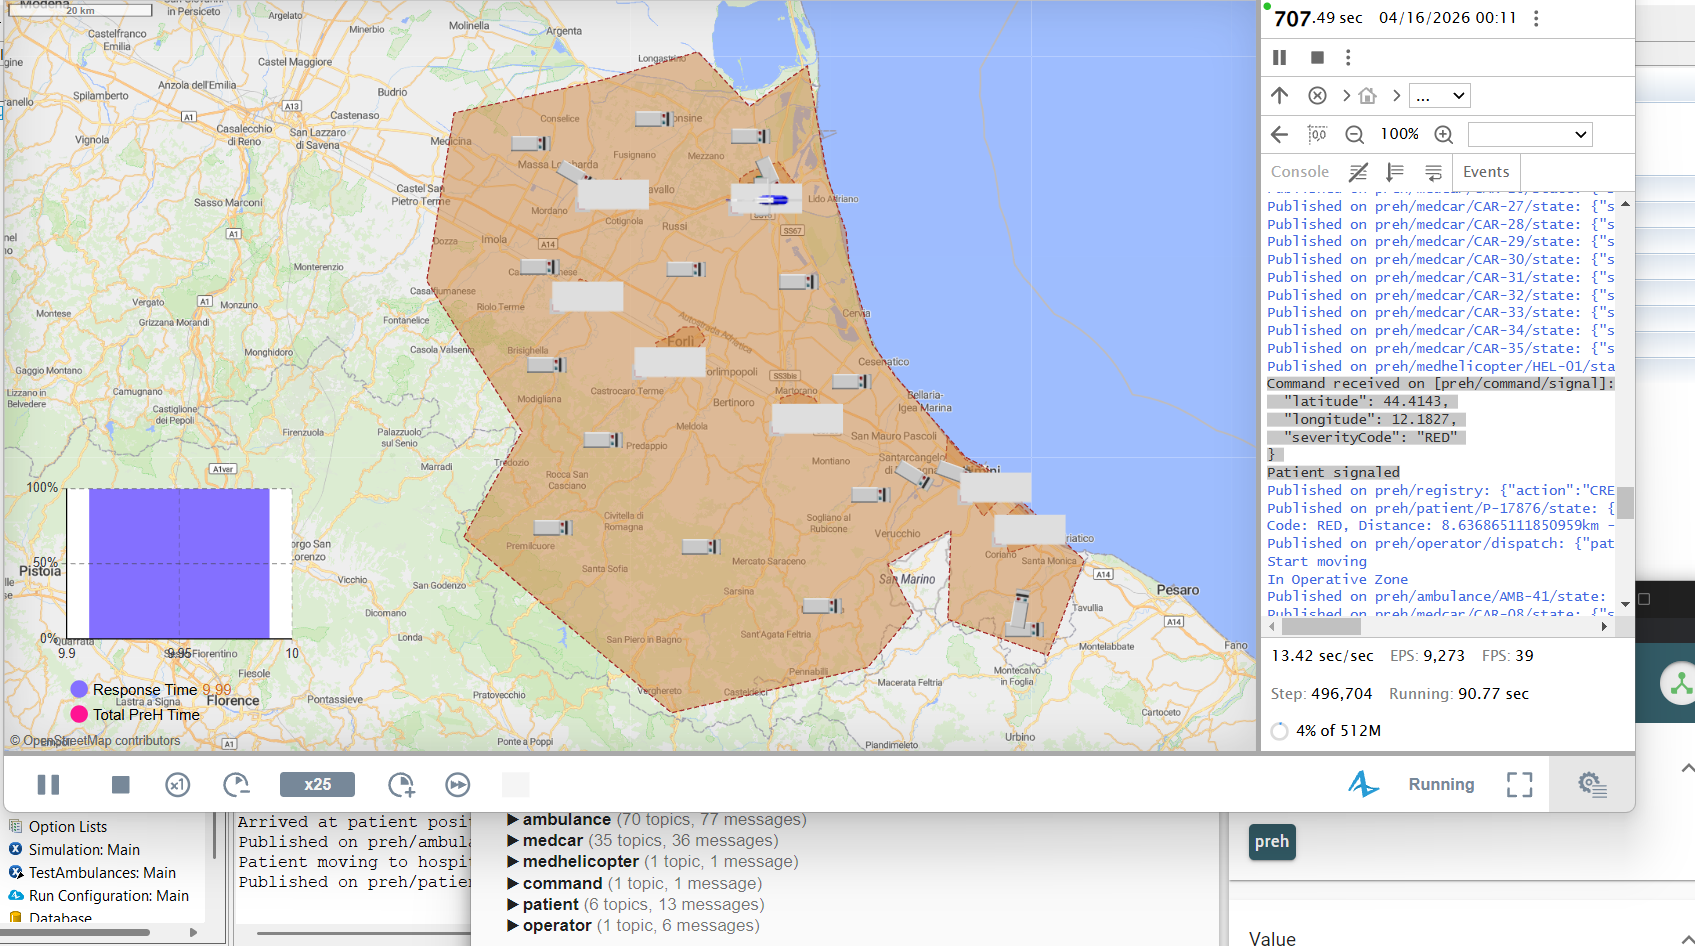
\includegraphics[width=1\textwidth]{img/mqttexp1.png}
    \label{fig:mqttexp1}
    \caption{Istanziamento degli agenti tramite messaggi al broker e pubblicazione emergenza al topic \texttt{preh/command/signal}}
\end{figure}

\begin{figure}[H]
    \centering
    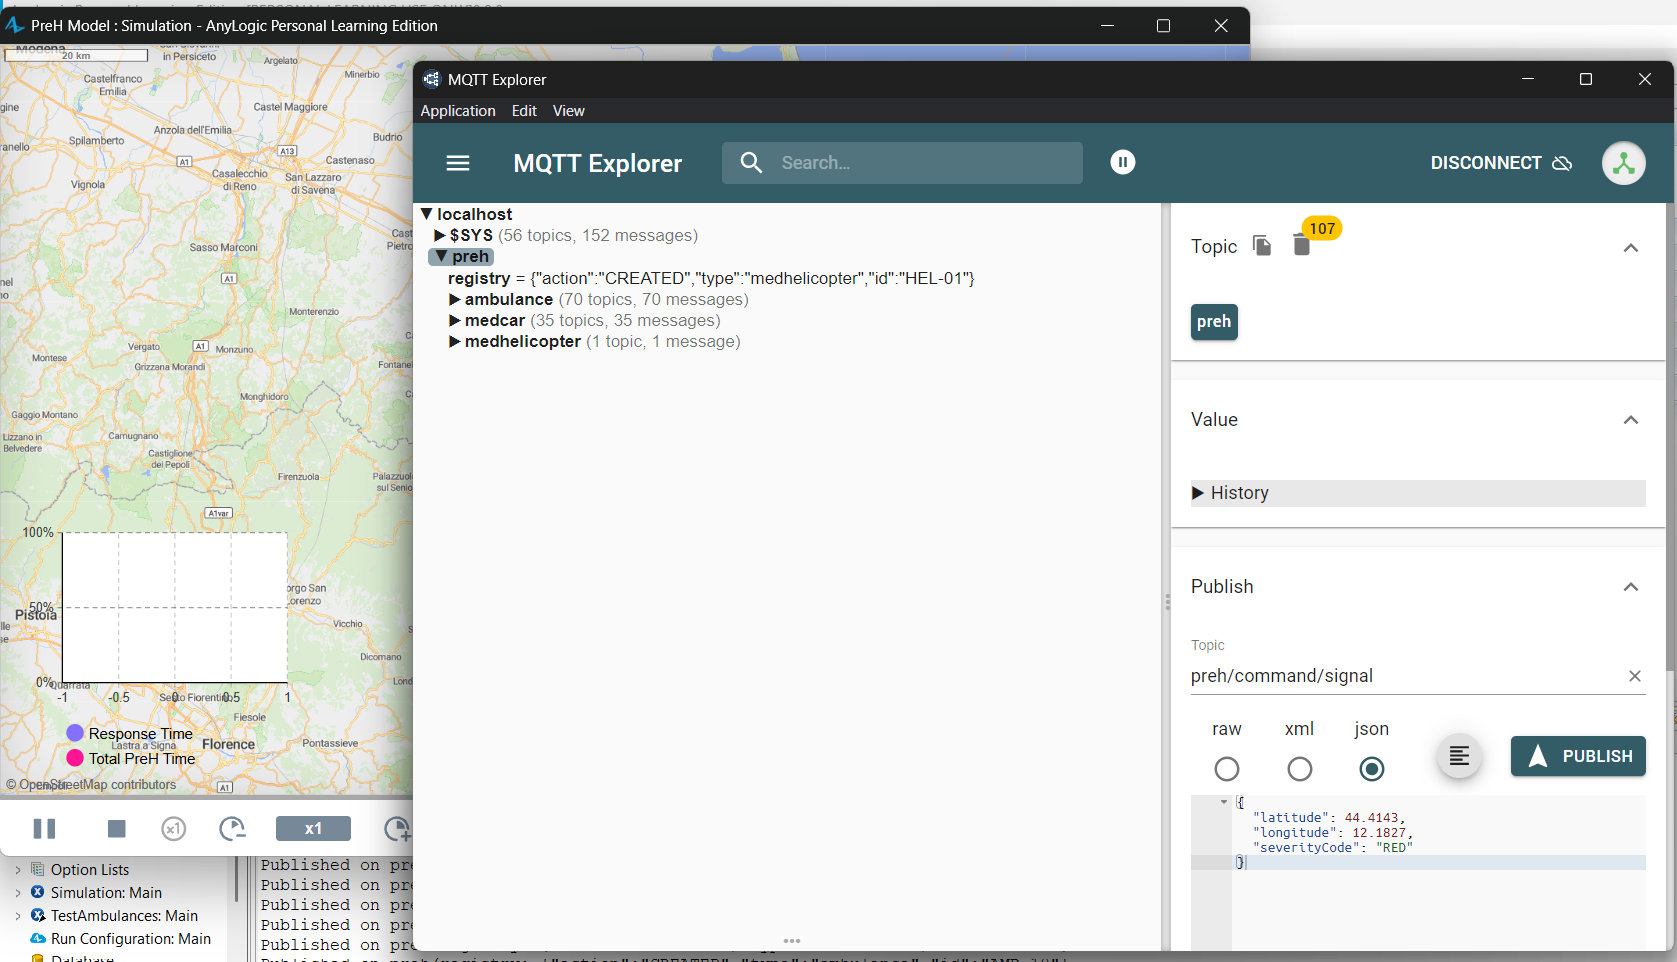
\includegraphics[width=1\textwidth]{img/mqttexp2.png}
    \label{fig:mqttexp2}
    \caption{Reazione della simulazione alla pubblicazione del messaggio ricevuto dal broker}
\end{figure}

Come è possibile vedere nella Figura \ref{fig:mqttexp1} e nella Figura \ref{fig:mqttexp2} è possibile
vedere che il meccanismo funziona. Questo risultato permette di rendere la simulazione ancora più manovrabile
dall'esterno.

\section{Conclusioni}
Quanto svolto ha dei limiti, la simulazione in primis tenta di fare le veci della realtà 
e non è possibile modellare tutte le complessità presenti. Inoltre l'applicazione AnyLogic
presenta alcuni difetti nel modellare alcuni aspetti reali tramite l'implementazione di cui dispone.
Nonostante queste problematiche, il tirocinio mi ha permesso molto sul mondo della simulazione
e di applicare quanto visto nel corso della laurea triennale, come il protocollo MQTT, Java e principi di
ingegneria del software. Inoltre, il protocollo ODD ha permesso di rendere più fruibile anche la creazione e la relativa documentazione
del modello creato, rendendolo più un lavoro di design che di effettiva implementazione. 
Il protocollo potrà essere valido in futuro anche per testare e verificare anche la comprensione del dominio
e di utilizzare meccanismi di predizione che potrebbero basarsi su questo paradigma.

\begin{thebibliography}{99}

\bibitem{evans2004domain}
E.~Evans, 
\emph{Domain-Driven Design: Tackling Complexity in the Heart of Software}.
\newblock Addison-Wesley, 2004.

\bibitem{grimm2006standard}
V.~Grimm, U.~Berger, F.~Bastiansen, S.~Eliassen, V.~Ginot, J.~Giske, J.~Goss-Custard, T.~Grand, S.~K. Heinz, G.~Huse, et~al.,
\newblock ``A standard protocol for describing individual-based and agent-based models,''
\newblock \emph{Ecological Modelling}, 2006.

\bibitem{grimm2010odd}
V.~Grimm, U.~Berger, D.~L. DeAngelis, J.~G. Polhill, J.~Giske, and S.~F. Railsback,
\newblock ``The ODD protocol: A review and first update,''
\newblock \emph{Ecological Modelling}, 2010.

\bibitem{minerva2020digital}
R.~Minerva, G.~M. Lee, and N.~Crespi,
\newblock ``Digital Twin in the IoT Context: A Survey on Technical Features, Scenarios, and Architectural Models,''
\newblock \emph{Proceedings of the IEEE}, 2020.

\bibitem{ricci2022web}
A.~Ricci, A.~Croatti, S.~Mariani, S.~Montagna, and M.~Picone,
\newblock ``Web of Digital Twins,''
\newblock \emph{ACM Transactions on Internet Technology}, 2022.

\bibitem{ricci2022pervasive}
A.~Ricci, A.~Croatti, and S.~Montagna,
\newblock ``Pervasive and Connected Digital Twins---A Vision for Digital Health,''
\newblock \emph{Computing in Science \& Engineering}, 2022.

\end{thebibliography}

\end{document}